
% Eigener Beitrag: Beschreibung, Begründung, Aufzeigung, Methode, Fazit

\chapter{Social Engineering}
\label{sec:socialengineering}

\section{Begriffserklärung}
\label{sec:socialengineering:begriffserklaerung}
Zur Erklärung des Begriffs des Social Engineering zeigt man am besten Beispiele auf:

\begin{quote}
	Hallo! Ich bin neu hier, wie komme ich nochmal ins Wifi? \footcite{Social_Engineering_Wenn_die_Gefahr_im_Anzug_kommt__t3n_2015-04-26}
\end{quote}

So einfach kann ein Angriff durch ein Social Engineer aussehen. In dem Beispiel wird versucht sich eine Dienstleistung zu erschleichen. Es gibt keine "`Hacks"' im eigentlichen Sinne. Niemand hängt sich ins Wireless rein, analysiert den Datenverkehr und versucht das Passwort zu knacken.

Angriffe können auch komplexer sein. Man stelle sich ein Unternehmen in Zürich vor, in welches Lastwagen einfahren. Oft haben Lastwagenfahrer ihren Namen auf einem Schild an der Frontscheibe aufgeschrieben. Sobald sich das Tor öffnet und der LKW einfährt, kann man dem Lastwagen nachrennen und den Namen des Fahrers rufen. So kommt man an den Sicherheitsbeamten am Tor vorbei. 
Der Angreifer möchte nun in die Abteilung Forschung \& Entwicklung. Er fragt eine Mitarbeiterin nach dem Weg, mit der Begründung, dass er von einer Tochterfirma in Basel kommt und die Wegbeschreibung am Empfang wohl falsch verstanden hätte. Die Mitarbeiterin gibt bereitwillig Auskunft.
Beim Gebäude der Abteilung Forschung \& Entwicklung ist die Türe abgeschlossen. Nun wartet der Angreifer mit Sicht auf die Türe, bis ein Mitarbeiter dort eintritt. Mit diesem zusammen betritt er das Gebäude. 
Der Angriff lässt sich nun beliebig weiterführen. Vielleicht hängt irgendwo eine Liste mit Telefonnummern oder ein Mitarbeiter hat Notizen an seinem Bildschirm angeklebt mit welchen der Angreifer weiterarbeiten kann. \footcite{Beispiel_fr_einen_Social_Engineering_Angriff_Social_Engineering_-_Manipulation_2015-04-26}

Dieser Angriff nutzt verschiedene Schwachstellen aus. Allen gemein ist dass sie nichts direkt mit Informatik zu tun haben und deshalb in der Kategorie des Social Engineering anzusiedeln sind. Dies wäre der Name an der Windschutzscheibe des LKW's, die Hilfsbereitschaft der Mitarbeiter oder dass offenhalten einer abgeschlossenen Türe für einen Kollegen.

Social Engineering muss nicht immer krimineller Natur sein. das nächste Kapitel setzt sich mit dieser Thematik auseinander.

\section{Typen von Social Engineers}
Social Engineering kann verschiedene Formen annehmen. Diese können bös- oder gutwillig sein. Folgend eine nicht abschliessende Liste von Aktivitäten\footcite{human_hacking} welche mit Social Engineering in Bezug gebracht werden kann:

\begin{itemize}
\item Hacker
\item Spione
\item Identitätsdiebe
\item Verärgerte Angestellte
\item Penetrationstester
\item Regierungen
\item Ärzte, Psychologen, Rechtsanwälte
\item Personalvermittler
\item Verkaufspersonal 
\end{itemize}

Gemeinsam haben diese Jobs, dass sie sich mit der Domäne, in welchen sie agieren, auskennen müssen, viele Informationen zu sammeln haben und ein geschickter Umgang mit Kommunikation besitzen müssen.

\textit{Spione} und \textit{Identitätsdiebe} müssen Informationen über das Ziel sammeln, sich in eine Rolle hineinversetzten und auch Kommunizieren wie diese.

\textit{Verärgerte Angestellte} können grossen Schaden anrichten. Mister X wird entlassen. Beim Gespräch mit dem Chef zeigt er sich verständnisvoll. Sobald er am Arbeitsplatz zurückkehrt beginnt er wichtige Daten zu löschen oder gibt diese weiter. Mister X darf sich nichts anmerken lassen. Muss Kommunizieren wie er es immer tut und den anderen Mitarbeitern etwas vortäuschen.
\textit{Penetrationstester} untersuchen Software auf Fehler. Dabei müssen sie sich in die Lage eines Hackers versetzen, so denken und handeln, wie dieser es tut. Dies umfasst deshalb die gleichen Kompetenzen eines Hackers.

\textit{Regierungen}, \textit{Ärzte}, \textit{Psychologen} und \textit{Rechtsanwälte} haben eines gemeinsam haben. Eine gute Kommunikation. Wie verkaufe ich etwas? Wie vermittle ich dem Volk etwas damit es nicht falsch verstanden wird? Wie überbringe ich eine schlechte Botschaft möglichst sanft? All diese Fragen bedienen sich dem Arsenal des Social Engineerings.

\textit{Personalvermittler} und \textit{Verkaufspersonal} müssen über ihre Produkte und die Kunden wichtige Informationen besitzen, sowie gutes Verhandlungsgeschick besitzen.

Es wurde an Beispielen gezeigt, dass Informationen sammeln und eine geschickte Kommunikation zwei Schlüsselaspekten des Social Engineerings darstellen. Das erste Thema welches nun genauer betrachtet wird ist das Sammeln von Informationen.

\section{Informationssammlung}
Informationen sind das Fundament des Social Engineering. Ist die Basis schief, kann man keine geschickte Angriffe durchführen. Die Aufgabe der Informationssammlung gliedert sich dabei in zwei Bereiche. Die Beschaffung und die Organisation der Daten. Jede erdenkliche Quelle von Informationen sollte dabei durchsucht werden. Ein Haufen von undurchsuchbaren Daten nützt jedoch dem besten Social Engineer nichts. Deshalb müssen diese geordnet und durchsuchbar gegliedert werden.

\subsection{Quellen}
Ein Social Engineer ist nicht wählerisch in der Auswahl seiner Informationsquellen. Webseiten, Blogs, Suchmaschinen, Whois-Abfragen, Öffentliche Server, Social Media und öffentliche Berichte ist eine nicht abschliessende Liste von verlässlichen Datenquellen. 

Man muss sich jedoch nicht nur auf online Medien beschränken. Durch Observation von Personen, Fahrzeugen oder Gebäuden können wertvolle Informationen gewonnen werden. Zu guter letzt darf sich ein Social Engineer auch nicht zu schade sein Abfälle zu durchwühlen. Diese Aktivität wird auch liebevoll Dumpster-Diving oder Garbage-Picking genannt. 

Es ist verblüffend, wie viele Wertvolle Informationen im Müll landen. Checks, Gehaltslisten, Telefonnummern, Namen oder sogar Passwörter werden oft im Abfall entsorgt. Auch wenn sich die Opfer mühe geben und die Unterlagen zuerst durch einen Dokumentenschredder unkenntlich machen nützt dies nichts. Nach ein paar Stunden kann man die Streifen zu einem ganzen Papier zusammenfügen. 

\begin{figure}[htb]
  \begin{subfigure}[b]{.45\linewidth}
    \centering
    
\includegraphics[width=0.5\linewidth]{images/shredded-paper.jpg}
    \caption{Geschreddertes Dokument}
    \label{fig:socialengineering:informationssammlung:quellen:schreddern:subfigures:a}
  \end{subfigure}%
  \begin{subfigure}[b]{.45\linewidth}
    \centering
    
\includegraphics[width=0.5\linewidth]{images/reassembled-shredded-paper.jpg}
    \caption{Zusammengesetztes Dokument}
    \label{fig:socialengineering:informationssammlung:quellen:schreddern:subfigures:b}
  \end{subfigure}
  \caption{Schreddern eines Dokumentes}
  \label{fig:socialengineering:informationssammlung:quellen:schreddern:figures}
\end{figure}

Das einzig verlässliche ist ein Zwei-Wege-Schredder. Solch unkenntlich gemachte Informationen lassen sich nicht mehr zusammenfügen.

\begin{figure}[H]
  \centering
  
\includegraphics[width=0.4\textwidth]{images/two-way-shredded-paper.jpg}
  \caption[Test image for television]{Zwei-Wege geschreddertes Dokument}
  \label{fig:socialengineering:informationssammlung:quellen:zwei-wege-schreddern}
\end{figure}

\subsection{Datenorganisation}
Beim der Sammlung können schnell ein paar Hundert Megabytes an Daten angehäuft werden. Dann stellt sich die Frage wie diese in eine ordentliche Form gebracht werden können. 

Hier gibt es Tool die einen Social Engineer in seiner Sammelwut unterstützen. Wichtige Aspekte einer solchen Software ist es, dass sie einfach zu bedienen und übersichtlich ist. Denn man wird viel Zeit mit ihr verbringen. Natürlich muss sie auch mit grossen Datenmengen umgehen können und jegliche Formen von Daten unterstützen. Dies geht über Text, Bildern bis zu PDF und weiteren Dateien. 

Ein einfaches Tool stellt BasKet dar. Es ist ein OpenSource Tool welches unter der GNU GPL v2 Lizenz betrieben wird und läuft mit Windows, Mac und Linux. Wie der Name bereits aussagt ist es ein Korb für die Ablage von jeglichen Daten.

\begin{figure}[htb]
  \centering
  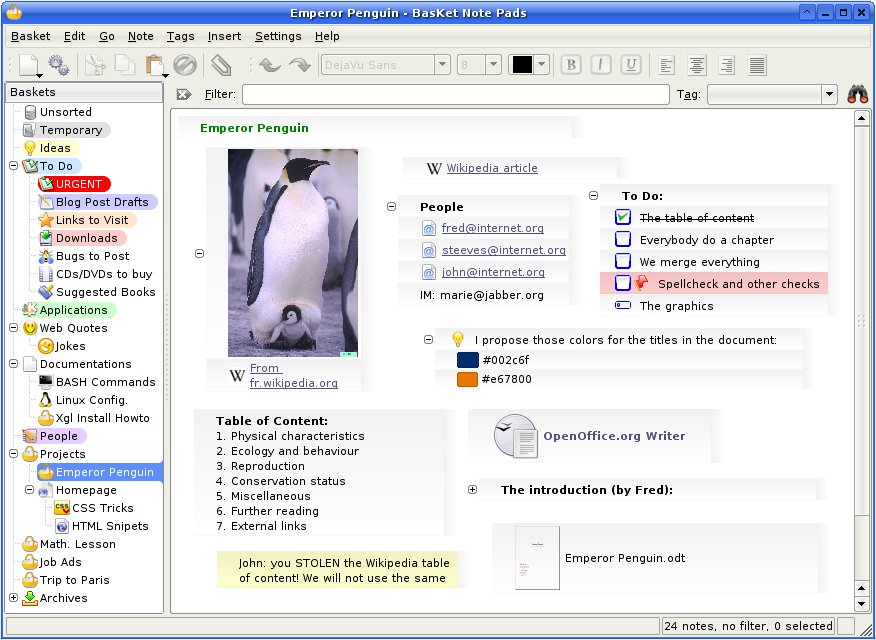
\includegraphics[width=0.8\textwidth]{images/basket.png}
  \caption[Test image for television]{BasKet ermöglicht die einfache Ablage von jeglichen Informationen}
  \label{fig:socialengineering:informationssammlung:datenorganisation:basket}
\end{figure}

Wenn man in einem Team arbeitet, muss eine gemeinsame Ablage der Daten möglich sein. Hier schafft das Programm Dradis abhilfe. Es läuft unter der gleichen Opensource Lizenz wie BasKet und ist auch für die selben Betriebsysteme verfügbar. 

Bei Dradis handelt es sich um ein Webapplikation. Das ganze Team kann dabei auf einer Webseite kollaborieren.

\begin{figure}[htb]
  \centering
  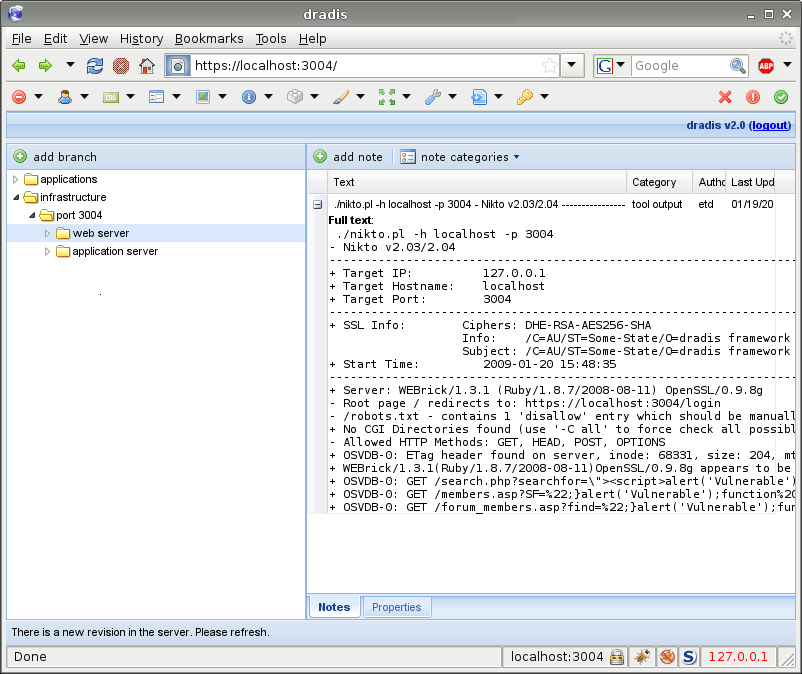
\includegraphics[width=0.8\textwidth]{images/dradis.png}
  \caption[Test image for television]{Mit Dradis können Teams zusammen arbeitent}
  \label{fig:socialengineering:informationssammlung:datenorganisation:basket}
\end{figure}

\section{Kommunikation}
Kommunikation ist eine wichtige Waffe für einen Social Engineer. Dabei geht es darum, Informationen von einer Person zur nächsten zu transferieren. Dies kann verbal, oder über visuelle Effekte, Berührungen, Gerüche oder digital sein.
Für den Social Engineer ist es dabei wichtig, wie die Informationen übermittelt werden, und zwar so, wie seine Absichten sind.
Ein Arzt muss eine schlechte Nachricht möglichst sanft übermitteln. Möchte man hingegen einem Opfer Informationen entlocken, muss man Sympathien aufbauen.

Die Schwierigkeit bei der Kommunikation liegt darin, das Gegenüber richtig zu lesen und die Botschaft so zu überbringen, dass sie die richtige Wirkung erzielt.
Dies wird versucht über Kommunikationsmodelle zu beschreiben.

\subsection{Kommunikationsmodell}
Kommunikationsmodelle versuchen die Kommunikation zu beschreiben. Also was Kommunikation ist und wie sie funktioniert. 

Ein Gesprächspartner hat immer seine eigene Realität und Ansichtsweisen. Dies kann dazu führen, dass das Gesagte nicht immer gleich interpretiert wird. 

Im Jahre 1947 entwickelten Claude Shannon und Warren Weaver das Shannon-Weaver-Modell, welches auch "`Mutter aller Modelle"' genannt wird.

\begin{figure}[H]
  \centering
  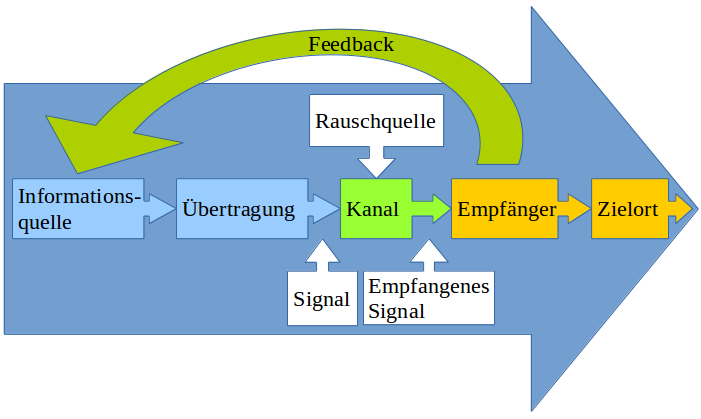
\includegraphics[width=0.8\textwidth]{images/shannon-weaver-model.png}
  \caption[Test image for television]{Kommunikationsmodell nach Shannon und Weaver}
  \label{fig:socialengineering:Kommunikation:Kommunikationsmodell:shannon-weaver-model}
\end{figure}

Der Ablauf einer Kommunikation lässt sich folgendermassen beschreiben:
\begin{itemize}
\item Informationsquelle: Quelle, welche eine Botschaft generiert.
\item Übertragung: Übermittler, der die Botschaft in Signale umsetzt.
\item Kanal: Ein Kanal, über den die Botschaft übermittlet wird. Dies kann über die sechs Sinne (sehen, hören, fühlen riechen oder schmecken) geschehen, oder über non-verbale Wege, wie zum Beispiel die Körpersprache.
\item Empfänger: Empfänger der Botschaft.
\item Feedback: Der Empfänger gibt der Quelle ein Feedback.
\item Zielort: Eventuell ist der Empfänger noch nicht die Endstation der Botschaft. Deshalb kann sie von ihm noch an einen Zielort weitergetragen werden.
\end{itemize}
Zusätzlich gibt es eine Rauschquelle, welche den Kanal stören kann. Das Signal ist dabei die Nachricht, wie sie von der Informationsquelle gedacht ist und das empfangene Signal ist die Botschaft, wie sie vom Empfänger interpretiert wird.

\subsection{Kommunikationsmodelle nutzen für das Social Engineering}
Für jeden Angriff muss sich ein Social Engineer sein Kommunikationsmodell festlegen. 

Um dies an einem praktischen Beispiel zu Zeigen stellt man sich ein Empfang vor. Durch Nachforschung hat man herausgefunden, dass der die PC's der Empfangsdame kein rechte Besitzt, somit für einen Angriff uninteressant ist. Der PC des Chefs jedoch hat erhöhte privilegien wodurch sich eine Schwachstelle offenbart. Der Chef hat auch einen Drucker, die Empfangsdame nicht.

Nun bereitet man einen USB-Stick vor, welcher ein Virus in das System einspeist, sobald er an den PC angeschlossen wird. Zusätzlich kopiert man noch ein PDF File mit ein einem Lebenslauf auf den Stick. 

Mit dieser Vorbereitung betritt man die Firma, geht zum Empfang und Teilt der Dame mit, dass man soeben den Lebenslauf mit Kaffee bekleckert hat. Man fragt, ob sie ihn nicht nochmals vom USB-Stick ausdrucken könne. Bereitwillig nimmt die Empfangsdame den Stick entgegen, geht zum Chef und fragt ihn, ob er den Lebenslauf ausdrucken kann. Dieser willigt ein und der Angriff ist erfolgreich.

Analysiert man das Kommunikationsmodell zu diesem Angriff, so sieht dies folgendermassen aus:
\begin{itemize}
\item Informationsquelle: Beobachtung und die Informationssammlung des Social Engineers.
\item Übertragung: Der Angreiffer
\item Kanal: Verbal
\item Empfänger: Die Empfangsdame
\item Feedback: Bereitwillige Einwilligung der Empfangsdame.
\item Zielort: Chef des Empfangs.
\end{itemize}

\section{Elizitieren}
Elizitieren steht dafür, jemandem etwas zu entlocken. Es versteht sich von selbst dass dies für jeden Social Engineer eine wichtige Angelegenheit darstellt. Man muss in der Lage sein, Fragen so zu gestalten, dass Menschen aus sich herauskommen und so stimmuliert werden, dass sie ein gewünschtes Verhalten einschlagen.

Einsetzen können diese Fähigkeit zum Beispiel Projektleiter, wenn sie mit Kunden kommunizieren, Polizisten, wenn sie verdächtige Verhören oder Hacker, wenn sie Informationen von Opfern erhalten möchten.

\subsection{Angriff auf die Firma XY Computing\footcite{human_hacking}}
Dieser Abschnitt zeigt ein Beispiel eines Angriffes auf. Man möchte mehr über eine Firma in Erfahrung bringen. Zu beginn muss man Informationen Sammeln. Auf der Webseite findet man heraus welche Produkte vertrieben werden und für was diese eingesetzt werden können. Ein Produkt wird in einem Magazin sehr gelobt. In dem Bericht wird der Mitarbeiter John Smith interviewt. Er ist der \Gls{cfoLabel} der Firma und verantwortlich für dieses Produkt.
Für sich selber legt man ein Pseudonym zu. Man wählt den Namen "`Paul Parker"' und bestellt ein paar fiktive Visitenkarten im Internet. 
Mit diesem Vorkehrungen geht man zu einem offenen Fest der Handelskammer in einer Bar. Dort sichtet man John Smith wie er mit einigen Reportern spricht. Als er sich aufmacht zur Bar zu gehen, schaut man dass man gleichzeitig dort ankommt. 

Paul: "`Na, auch den Geiern entkommen?"'

John schmunzelt: "`Sie sagen es, ich brauche einen Drink"'.

Paul zieht eine Visitenkarte hervor: "`Ich arbeite bei einer kleinen Importfirma als Einkaufsleiter"'

John überreicht seiner Seitens eine Vistenkarte: "`Ich bin John Smith, \Gls{cfoLabel} von XY Computing.

Paul: "`Ah, sie sind der Typ mit den Taschen voller Geld ... darum sind alle hinter Ihnen her. Was macht Ihre Firma eigentlich?"'

John beginnt über die Produkte zu sprechen. Als er über das zuvor recherchierte zu sprechen beginnt fällt man ihm ins Wort.

Paul: "`Ach ja, dieses Produkt kommt ja von \textit{Ihrer} Firma. Ich liebe das Teil. Ich habe im XYZ-Magazin gelesen, dass Sie damit einen absoluten Verkaufshit gelandet haben."'

John drückt den Rücken etwas durch: "`Wussten Sie, dass wir dieses Gerät im ersten Monat mehr verkauft haben als das davor und die nächsten fünf Produkte zusammen?"'

Paul: "`Oha - tja, und ich weiss auch warum. Ich habe nämlich selbst fünf Stück davon gekauft."'

Nach einigen weiteren Minuten findet man heraus, welche neue Buchhaltungssoftware die Firma soeben gekauft hat, dass der John soeben in den Ferien war und dass auch der \Gls{csoLabel} gleich für ein paar Tage in die Bahamas fliegt. Was bringen diese Infos einem Social Engineer? Für die Planung eines Angriffes können vertiefte Informationen über Produkte, Leute und Urlaubstermine entscheidend sein. Das Gespräch geht noch weiter.

Paul: "`Ich weiss, dass das vielleicht eine komische Frage ist, aber wir sind eine kleine Firma, und mein Chef hat mich beaftragt, mal Recherchen anzustellen und ein Sicherheitssystem für die Türen zu kaufen. Aktuell haben wir nur Schlüssel, aber er fand, dass so was wie \gls{glos:rfidLabel} vielleicht ganz gut ist. Sie wissen bestimmt, was bei Ihnen verwendet wird!"'

John: "`Ich habe keine Ahnung, ich habe dafür nur die Rechnungen gegengezeichnet. Ich weiss nur, dass wir diese schicke kleine Karte haben ..."'

Mit diesen Worten zog er seine Geldbörse heraus und zieht eine Karte heraus.

John: "`Ich glaube, das ist so ein \gls{glos:rfidLabel}-Ding, aber sonst weiss ich nur, dass ich mit meinem Portemonnaie vor dem kleinen Kasten rumwedeln muss, umd die Tür geht auf"'.
\\
\\
Einem normalen Menschen erscheinen die erhaltenen Informationen nutzlos. Ein Social Engineer kann sich daraus jedoch wesentliche Vorteile ziehen. Es wurden eine Liste an Details über Software, Leute und Urlaubstermine gesammelt sowie Informationen über die Sicherheitssysteme der Firma.
Möchte man sich Zutritt zum Gebäude verschaffen geht man zum Empfang und sagt dort, dass man eine \gls{glos:rfidLabel}-Box defekt ist und dass der \Gls{csoLabel} einem beauftragt hätte, bevor er in die Bahamas flog.

\subsection{Techniken}
Im vorhergegangen Kapitel wurde ein Angriffszenario aufgezeigt, welches verschiedene Techniken des Social Engineering enthält. Zu Begin ist eine gute Vorbereitung nötig. Im Gespräch mit dem \Gls{csoLabel} kam das Elizitieren zum Einsatz. 

Als John (der \Gls{csoLabel}) von seinem besten Produkt zu erzählen beginnt, zeigt Paul, dass er davon begeistert ist und unterschreicht dessen Genialität. Dadurch \textbf{appelliert} Paul (der Social Engineer) \textbf{ans Ego} von John, welcher sofort drauf einsteigt und weitere Informationen nachreicht.

Mit dem Satz "`Ach ja, dieses Produkt kommt ja von Ihrer firma. Ichliebe das Teil"' bekundet Paul ein \textbf{gegenseitiges Interesse}. Dieses ist ein wichtiger Aspekt des Elizitieren, da es sogar noch wirkungsvoller ist als das Ego des gegenübers anzukraulen.

Später im Gespräch nutzt Paul eine weitere Technik, indem er dem Gesprächspartner \textbf{Kenntnisse unterstellt}. "`Sie wissen bestimmt, was bei Ihnen verwendet wird!"' ist dabei der Schlüsselteil des Satzes. John weiss zwar die Antwort auf die Frage nicht, versucht jedoch trotzdem noch weiterzuhelfen, indem er seine \gls{glos:rfidLabel}-Karte hervorholt.

Die der ganze Angriff war deshalb so erfolgreich, da \textbf{Alkohol} mit im Spiel war. Nichts lockert die Lippen besser als Ethanol.

In der aufgeführten Attacke nicht verwendet, jedoch auch ziemlich erfolgreich ist es, wenn man seinerseits \textbf{Informationen freiwillig anbietet}. Dadurch nötigt man seinem Gegenüber, eine ähnlich wertvolle Angabe zu machen.

Die letzte Waffe, die das Elizitieren bietet ist es, wenn man selbst eine \textbf{absichtlich falsche Aussage trifft}. Dies regt den Stolz des Anderen an, da er die Aussage berichtigen kann, wodurch oft geheime Informationen weitergegeben werden.

\subsection{Grundsätzliches}
Beim Elizitieren gibt es drei Grundregeln: \textbf{Seien Sie natürlich}, \textbf{Schulen Sie sich selbst} und \textbf{seien Sie nicht gierig}. 

Wenn man nicht natürlich ist, kann das Gespräch schneller vorbei sein als es begonnen hat. 

Mit "`Schulen Sie sich selbst"' ist eine gute Vorbereitung gemeint. Man muss Informationen sammeln und deren Wert für das Gegenüber kennen. Es ist auch wichtig, dass man sich nie für mehr ausgibt, als man mit den gesammelten Informationen darstellen kann. Wenn das Opfer merkt, dass man etwas vorspielt, gibt er sicher keine weitere Informationen frei.

Natürlich hat man stets das Ziel, möglichst viele Informationen zu ergattern. Ist man jedoch zu gierig, kann es schnell gefährlich werden, da der Gesprächspartner den Angriff möglicherweise bemerkt.

Der grosse Vorteil der erwähnten Techniken ist, dass es oft nicht auffällt wenn man Opfer einer Attacke wird. Die Hürde ist zwar hoch, da man zum Teil direkt in Kontakt mit dem Opfer trifft, jedoch kann ein Meister des Elizitieren viele wertvolle Informationen ergattern, ohne entdeckt zu werden.

\section{Pretexting}
Die nächste Disziplin eines Sociala Engineers ist das Pretexting. Dabei schlüpft man in die Haut einer anderen Person und gibt sich für diejenige aus.

Im Kapitel \cref{sec:socialengineering:begriffserklaerung} wurde ein Angriffsszenario aufgezeigt. Der Pretext besteht in dem Fall daraus, dass sich der Eindringling als Mitarbeiter der Tochterfirma ausgibt. Als Vorbereitung ist hier eine ausführliche Recherche vor dem Angriff notwendig. Verstärkt werden kann der Pretext wenn der Social Engineer sich auch noch entsprechend kleidet. Man kann sich zum Beispiel mit einem grauen Overall und einem Schraubenziehen in der Tasche verkleidet als Supportmitarbeiter ausgeben.

Als wichtigste Regel gibt es zu beachten, dass der Pretext \textbf{so einfach wie möglich} gehalten werden soll. Muss man sich zu viel einprägen kann man auf Fragen in einem Gespräch keine konsistente Antworten geben. Dies merkt man als Gegenüber rasch und gibt somit keine Informationen mehr preis. Verschiedene Pretexte erfordern auch mehr Wissen als andere. Es ist einfacher sich als Briefmarkensammler auszugeben verglichen mit einem Atomforscher. 

Zusätzlich sollte der Pretext \textbf{sponatan wirken}. Wenn man zu viel nachdenken muss wird man innerlich unruhig. Zu vergleichen ist dies wie ein Sprung vom 10 Meter Sprungbrett in einen Pool. Wenn man oben steht und zu lange nachdenkt bekommt man Angst und springt nicht mehr.

Am Ende eines Angriffes ist es stets ratsam, einen \textbf{logischen Schluss oder Folgeauftrag} zu \textbf{erteilen}. Die Menschen mögen es, wenn sie Aufträge erteilt bekommen. Ein Arzt sagt nach der Behandlung nicht "`Wir sehen uns in vier Wochen wieder"'. Man zieht ein Schluss über das Gespräch und sagt dem gegenüber wie man verbleibt. Allfällige Auftrage müssen jedoch stets zum Pretext passen. Ist der Folgeauftrag wichtig für den Erfolg eines Angriffes ist es ratsam, wenn der Social Engineer selber Aktiv wird. Zum Beispiel wenn der Angegriffene Informationen an den Angreifer weitergeben soll ist es nicht ratsam zu sagen: "`Melden Sie sich am Monatag bei mir"'. Besser ist es "`Ich melde mich am Montag bei ihnen, wenn das recht ist"'. Dann läuft man nicht Gefahr, dass der Auftrag vergessen geht.

Hilfreich ist es, wenn man lokale \textbf{Dialekte und Redensarten} verwendet. In der Schweiz stösst man oft auf Abneigung, wenn man in Hochdeutsch spricht. In Amerika finden es viele Menschen sympathischer, wenn jemand einen britischen Akzept besitzt. Der Akzent muss dabei authentisch verkörpert werden können. Ist dies nicht möglich sollte er besser vergelassen werden, da der Gesprächspartner merkt dass ihm etwas vorgespielt wird. Es gibt diverse Studien die belegen, dass der Akzent einen wesentlichen Einfluss auf das Verhalten des zuhörers hat \footcite{Journal_of_Targeting_Measurement_and_Analysis_for_Marketing_2015-05-14}\footcite{The_Effect_of_Perceived_Regional_Accents_on_Individual_Economic_Behavior_2015-05-14}.

Schlussendlich muss der Pretext vorher ausgiebig geübt werden. Dies kann vor dem Spiegel getan werden, oder man nimmt sich dabei auf. Auch ratsam ist es, wenn man mit fremdene Leuten spricht und deren Reaktion beobachtet.

\section{Weitere Techniken}
Social Engineering ist, mehr als jede andere Angriffsart, eine sehr psychologische Angelegenheit. Es gibt deshalb noch viele andere Techniken, welche man sich zu nutzen machen kann. Nachfolgend noch eine nicht abschliessende Liste von weniger wichtigen, jedoch hilfreichen Fertigkeiten.

\subsection{Mikroexpressionen}
Vieles lässt sich au dem Gesicht des Gegenübers ablesen. Diese Mikroexpressionen zu deuten ist wichtig um weitere Schritte im Social Engineering zu planen.
Folgend einige Beispiele von Gesichtsausdrücken
\footcite{Anger_by_kwerfeldein_on_DeviantArt_2015-05-16}
\footcite{Ekman_-_Facial_Expressions_Foreign_Language_Flashcards_-_Cramcom_2015-05-16}
\footcite{Facial_expression_project_-_laughing_girls__Flickr_-_Photo_Sharing_2015-05-16}.

\begin{figure}[htb]
	\begin{subfigure}[b]{.30\linewidth}
		\centering
		
\includegraphics[width=0.5\linewidth]{images/mikroexpression-wut.jpg}
		\caption{Wut}
		\label{fig:socialengineering:weiteretechniken:mikroexpressionen:wut}
	\end{subfigure}%
	\begin{subfigure}[b]{.30\linewidth}
	  \centering
	  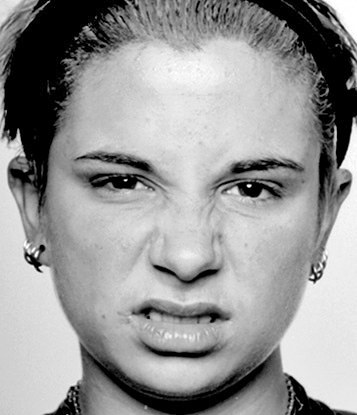
\includegraphics[width=0.5\linewidth]{images/mikroexpression-ekel.jpg}
	  \caption{Ekel}
	  \label{fig:socialengineering:weiteretechniken:mikroexpressionen:          ekel}
	\end{subfigure}
	\begin{subfigure}[b]{.30\linewidth}
		\centering
		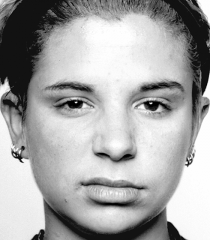
\includegraphics[width=0.5\linewidth]{images/mikroexpression-verachtung.png}
		\caption{Verachtung}
		\label{fig:socialengineering:weiteretechniken:mikroexpressionen:verachtung}
	\end{subfigure}
	\begin{subfigure}[b]{.30\linewidth}
		\centering
		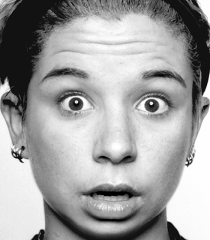
\includegraphics[width=0.5\linewidth]{images/mikroexpression-ueberraschung.png}
		\caption{Überraschung}
		\label{fig:socialengineering:weiteretechniken:mikroexpressionen:ueberraschung}
	\end{subfigure}
	\begin{subfigure}[b]{.30\linewidth}
		\centering
		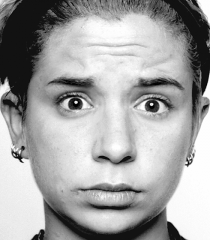
\includegraphics[width=0.5\linewidth]{images/mikroexpression-angst.png}
		\caption{Angst}
		\label{fig:socialengineering:weiteretechniken:mikroexpressionen:angst}
	\end{subfigure}
	\begin{subfigure}[b]{.30\linewidth}
		\centering
		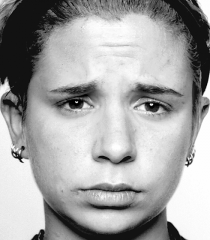
\includegraphics[width=0.5\linewidth]{images/mikroexpression-traurigkeit.png}
		\caption{Traurigkeit}
		\label{fig:socialengineering:weiteretechniken:mikroexpressionen:traurigkeit}
	\end{subfigure}
	\begin{subfigure}[b]{.30\linewidth}
		\centering
		
\includegraphics[width=0.5\linewidth]{images/mikroexpression-glueck.jpg}
		\caption{Glück}
		\label{fig:socialengineering:weiteretechniken:mikroexpressionen:glueck}
	\end{subfigure}
  \caption{Schreddern eines Dokumentes}
  \label{fig:socialengineering:weiteretechniken:mikroexpressionen}
\end{figure}

Zu beachten sind die Veränderungen der Augen, Stirn, Nase und den Mund. 